% -*- TeX-master: "main"; fill-column: 72 -*-

\newcommand{\fixttspace}{\hspace*{1pt}}

\section{Package syntax and semantics}
\label{sec:syntax}

In this section, we define the syntax and semantics of the Hierarchical
Model Composition package for SBML Level~3 Version~1.  We expound on the
various data types and constructs defined in this package, then in
\sect{examples}, we provide complete examples of using the constructs in
example SBML models.

% -----------------------------------------------------------------------------
\subsection{Namespace URI and other declarations necessary for using this package}
\label{xml-namespace}

Every SBML Level~3 package is identified uniquely by an XML namespace
URI.  For an SBML document to be able to use a given SBML Level~3
package, it must declare the use of that package by referencing its URI.
The following is the namespace URI for this version of the Hierarchical
Model Composition package for SBML Level~3 Version~1:
\begin{center}
\uri{http://www.sbml.org/sbml/level3/version1/comp/version1}
\end{center}

In addition, SBML documents using a given package must indicate whether
understanding the package is required for complete mathematical
interpretation of a model, or whether the package is optional.  This is
done using the attribute \token{required} on the \token{<sbml>} element
in the SBML document.  For the Hierarchical Model Composition package,
the value of this attribute may be set to \val{true} or \val{false},
depending on whether the constructs described in this package are used
in the model to change its mathematical meaning.

The following fragment illustrates the beginning of a typical SBML model
using SBML Level~3 Version~1 and this version of the Hierarchical Model
Composition package:

\begin{example}
<?xml version="1.0" encoding="UTF-8"?>
<sbml xmlns="http://www.sbml.org/sbml/level3/version1/core" level="3" version="1"
      xmlns:comp="http://www.sbml.org/sbml/level3/version1/comp/version1" comp:required="true">
\end{example}
    

% -----------------------------------------------------------------------------
\subsection{Primitive data types}
\label{new-primitive-types}

Section~3.1 of the SBML Level~3 specification defines a number of
primitive data types and also uses a number of XML Schema 1.0 data
types~\citep{biron:2000}.  We assume and use some of them in the rest of
this specification, specifically \primtype{boolean}, \primtype{ID},
\primtype{SId}, \primtype{SIdRef}, \primtype{UnitSId},
\primtype{UnitSIdRef}, and \primtype{string}.  The Hierarchical Model
Composition package also makes use of or defines other primitive types;
they are described below.


\subsubsection{Type \fixttspace\primtypeNC{IDREF}}
\label{primtype-idref}

Type \primtype{IDREF} is defined by XML Schema 1.0.  It is a character
string data type whose value is identical to an \primtype{ID} defined 
elsewhere in a referenced document, and has identical syntax.


\subsubsection{Type \fixttspace\primtypeNC{anyURI}}
\label{primtype-anyuri}
\label{primtype-uri}

Type \primtype{anyURI} is defined by XML Schema 1.0.  It is a character
string data type whose values are interpretable as URIs (\emph{Universal
  Resource Identifiers}; \citealt{harold:2001,w3c:2000}) as described by
the W3C document RFC~3986~\citep{rfc3986}.


\subsubsection{Type \fixttspace\primtypeNC{PortSId}}
\label{primtype-portid}

The type \primtype{PortSId} is derived from \primtype{SId} (SBML Level~3
Version~1 Core specification Section~3.1.7) and has identical syntax.
The \primtype{PortSId} type is used as the data type for the identifiers
of \Port objects (Section~\ref{port-class}) in the Hierarchical Model Composition
package.  The purpose of having a separate type for such identifiers is
to enable the space of possible port identifier values to be separated
from the space of all other identifier values in SBML.  The equality of
\primtype{PortSId} values is determined by an exact character sequence
match; i.e., comparisons of these identifiers must be performed in a
case-sensitive manner.


\subsubsection{Type \fixttspace\primtypeNC{PortSIdRef}}
\label{primtype-portidref}

Type \primtype{PortSIdRef} is used for all attributes that refer to
identifiers of type \primtype{PortSId}.  This type is derived from
\primtype{PortSId}, but with the restriction that the value of an
attribute having type \primtype{PortSIdRef} must match the value of a
\primtype{PortSId} attribute in the relevant model;  in other words, the value of
the attribute must be an existing port identifier in
the referenced model.  As with \primtype{PortSId}, the equality of
\primtype{PortSIdRef} values is determined by exact character sequence
match; i.e., comparisons of these identifiers must be performed in a
case-sensitive manner.


% -----------------------------------------------------------------------------
\subsection{The extended \class{SBML} class}
\label{sbml-class}
\label{listofmodeldefinitions-class}
\label{listofexternalmodeldefinitions-class}

The top level of an ``SBML document'' is a container whose structure is
defined by the object class \SBML in the SBML Level~3 specification.  In
Level~3 Core, this container can contain only one model, an object of
class \Model.  The Hierarchical Model Composition package allows SBML
documents to contain \emph{more} than one model.

To explain how this is accomplished, we first need to introduce some
terminology.  In the approach taken here, we make a distinction between
(a) the definition of a model, before it is actually used anywhere, and
(b) its actual use:

\begin{itemize}

\item The term \emph{model definition} refers to the former case; that
  is, the definition of a model, before it is used.  A model definition
  is akin to a Platonic ideal: it may be a complete model in and of
  itself, but until it is instantiated, it exists only as a concept.

\item The term \emph{submodel} refers to actual use of a model
  definition.  A submodel is an instantiation or instance of a
  previously-defined model: it is the realization of that model inside
  another model.  From the perspective of the model that contains this
  submodel, the model definition has come into being, and now exists as
  something that can be used (and possibly modified and adapted).

\end{itemize}

% [MH] Took this out because it wasn't clear that it was needed:
% 
% The potentially arbitrary nesting possible in model composition adds an
% additional wrinkle to the model definition/submodel distinction.  If the
% model directly containing a given submodel is the \Model object of the
% SBML document, then the submodel has been fully instantiated.  However,
% if the containing model is instead \emph{another} model definition (call
% it ``M''), the submodel becomes part of that larger model definition,
% but has \emph{not} been fully instantiated in the SBML document.  The
% submodel only becomes fully instantiated when the model definition
% (``M'') is itself instantiated in the top-level \Model object of an SBML
% document.

It may be helpful to contrast these terms with those in other
approaches to model composition.  Some approaches call the model
definitions themselves the ``submodels''.  We avoid that usage because,
in the present formulation, model definitions must be valid \Model
objects in and of themselves, and might never appear inside other models
in the SBML document where they are defined.  (This might be the
situation, for example, if the document defines multiple models purely
to serve as a sort of component library used by other files.)  We
reserve the term ``submodel'' specifically for the \emph{instance of a
  model inside a containing model}.  Another term used in other schemes
is ``model template'', which is close to what is intended by ``model
definition'' here, but ``template'' implies something that is incomplete
and needs to be filled in.  While this is possible in the approach
described here, it is not required; for example, in model aggregation,
several complete working models may be integrated to form a larger
whole.  We therefore eschew the term ``model template'' in favor of
\emph{model definition}.

\begin{figure}[b]
  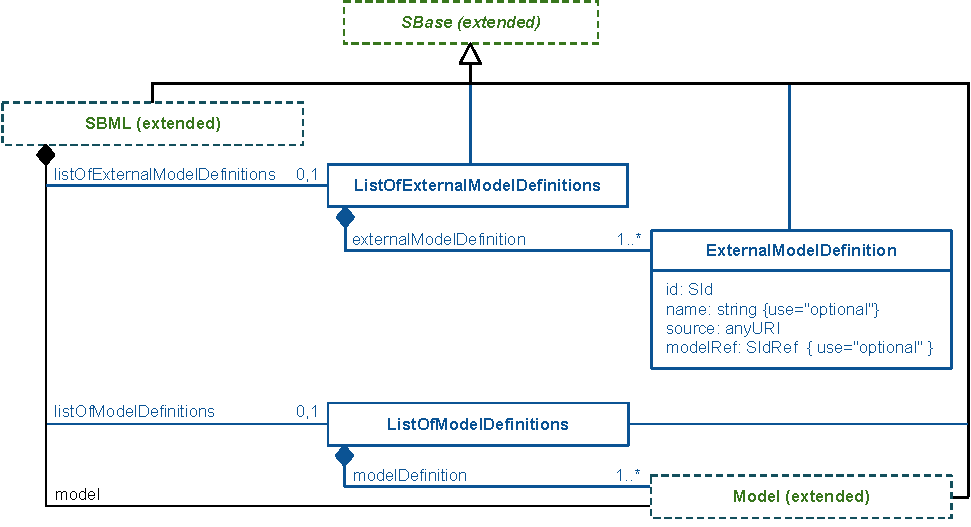
\includegraphics{figs/hierarchical-sbml}
  \caption{The definitions of the extended \SBML class as well as the
    new classes \ListOfModelDefinitions,
    \ListOfExternalModelDefinitions, and \ExternalModelDefinition.  The
    extended \Model class is defined in \sect{model-class}.}
  \label{hierarchical-sbml-uml}
  \label{sbml-uml}
\end{figure}

\fig{hierarchical-sbml-uml} gives the definition of the extended
\SBML class that ties these different components together; it also
provides the definition of \ExternalModelDefinition.  Readers familiar
with the \SBML class in SBML Level~3 Core will notice that this package
adds two new lists, \token{listOfModelDefinitions} of class 
\ListOfModelDefinitions and \token{listOfExternalModelDefinitions} 
of class \ListOfExternalModelDefinitions.  The class diagram
also makes concrete the notions described above, that model definition
objects are not ``owned'' by any other model (they can be instantiated
anywhere, even by models in other files) and that they exist outside the
\Model class entirely.

\fig{hierarchical-sbml-uml} also makes clear how model definitions
\emph{are} \Model objects.  At the same time, the scheme preserves the
aspect of core SBML Level~3 in which a single \Model object appears at
the top level of an SBML document.  As will become when we define
\Model, submodels appear inside \Model objects.  This is a key feature
of the design described above; namely, when the top-level model
references submodels, the submodels are instantiated, whereas when a
model definition references submodels, the submodels are simply part of
that model definition---they are not instantiated until the model
definitions themselves are instantiated.

Finally, to give a more intuitive sense for how the pieces fit together,
\fig{hierarchy} below shows a template structure of an SBML document
with both a \token{listOfModelDefinitions} and
\token{listOfExternal\-Model\-Definitions}, as well as a list of \Submodel
objects inside the \Model object.

\newcommand{\sayOptional}{\raisebox{0pt}[0pt][0pt]{\bigg\} \textrm{\emph{optional}}}}

\begin{figure}[hbt]
  \begin{tt}
    \examplespacing
    \small
    \fcolorbox{sbmlgray}{extremelylightgray}{%
      \begin{minipage}{\textwidth - 12pt}
        \begin{tabbing}
\=xx\=xx\=xx\=xx\=\kill
\+\>
<?xml version="1.0" encoding="UTF-8"?>\\
<sbml xmlns="http://www.sbml.org/sbml/level3/version1/core" level="3" version="1"\\
\>\>\>xmlns:comp="http://www.sbml.org/sbml/level3/version1/comp/version1" comp:required="true">\\[3pt]
\><model id="My\_Model">\\
\>\><comp:listOfSubmodels>\\
\>\>\>\textrm{\emph{one or more}} <comp:submodel> \ldots\ </comp:submodel> \textrm{\emph{elements}}  \` \sayOptional\\
\>\></comp:listOfSubmodels>\\
\></model>\\[3pt]
\><comp:listOfModelDefinitions>\\
\>\>\textrm{\emph{one or more}} <comp:modelDefinition> \ldots\ </comp:modelDefinition> \textrm{\emph{elements}}  \` \sayOptional\\
\></comp:listOfModelDefinitions>\\[3pt]
\><comp:listOfExternalModelDefinitions>\\
\>\>\textrm{\emph{one or more}} <comp:externalModelDefinition> \ldots\ </comp:externalModelDefinition> \textrm{\emph{elements}}  \` \sayOptional\\
\></comp:listOfExternalModelDefinitions>\\[3pt]
</sbml>
        \end{tabbing}
      \end{minipage}
    }
  \end{tt}
  \vspace*{-2pt}
  \caption{Example of a skeleton SBML Level~3 document containing the
    possible top-level constructs defined by the Hierarchical Model
    Composition package.}
\label{hierarchy}
\end{figure}



\subsubsection{The lists of internal and external model definitions}

As shown in \fig{sbml-uml}, \token{listOfModelDefinitions} and
\token{listOfExternalModelDefinitions} are children of an extended \SBML
object.  Like other \textsf{\textbf{ListOf\rule{0.15in}{0.5pt}}} classes
in SBML, the \ListOfModelDefinitions and \ListOfExternalModelDefinitions
are derived from \SBase (more specifically, the extended \SBase class
defined in \sect{extended-sbase-class}).  They inherit \SBase's
attributes \token{metaid} and \token{sboTerm}, as well as the
subcomponents for \Annotation and \Notes, but they do not add any
especial attributes of their own.

If a model from an external SBML document is needed, it can be
referenced with an \ExternalModelDefinition object
(\sect{externalmodeldefinition-class}).  The
\ListOfExternalModelDefinitions container gathers all such references.
It is derived from \SBase but adds no especial attributes of its own.
Like the other \textsf{\textbf{ListOf\rule{0.15in}{0.5pt}}} classes, it
inherits the attributes \token{metaid} and \token{sboTerm}, as well as
the subcomponents for \Annotation and \Notes, that most SBML components
have.


\subsubsection{The \class{ExternalModelDefinition} class}
\label{externalmodeldefinition-class}

To describe model definitions contained in external documents, the
Hierarchical Model Composition package uses a separate object class
(\ExternalModelDefinition), defined in \fig{hierarchical-sbml-uml}.  In
the sense being used here, \ExternalModelDefinition objects are model
definitions---in and of themselves, they are definitions of models but
not \emph{uses} of those models.  The \ExternalModelDefinition provides
a way to declare and identify them so that \Model objects in the 
present SBML document can use them in \Submodel objects.

\ExternalModelDefinition contains two required attributes
(\token{source} and \token{id}) and three optional attributes
(\token{modelRef}, \token{md5} and \token{name}).  These attributes are
explained below.


\paragraph{The \fixttspace\token{id} and \fixttspace\token{name} attributes}

The \token{id} attribute serves to provide a handle for the external
model reference so that \Submodel objects can refer to it.  (Crucially,
it is \emph{not} the identifier of the model being referenced; rather,
it is an identifier for this \ExternalModelDefinition object within the
current SBML document.)  The \token{id} attribute takes a required value
of type \primtype{SId}, and must be used as described in \sect{namespaces}.  

\ExternalModelDefinition also has an optional \token{name} attribute, of
type \primtype{string}.  The \token{name} attribute may be used
in the same manner as other \token{name} attributes on SBML Level~3 Core
objects; see Section~3.3.2 of the SBML Level~3 Version~1 Core
specification for more information.


\paragraph{The \fixttspace\token{source} attribute}

The required attribute \token{source} is used to locate the SBML
document containing an external model definition.  The value of this
attribute must be of type \primtype{anyURI} (see \sect{primtype-uri}).
Since URIs may be either URLs, URNs, or relative or absolute file
locations, this offers flexibility in referencing SBML documents.  In
all cases, the \token{source} attribute value must refer specifically to
an SBML Level~3 Version~1 document; prior Levels/Versions of SBML are
not supported by this package.  The entire file at the given location is
referenced.  The \token{source} attribute must have a value for every
\ExternalModelDefinition instance.

Here are some examples of different \token{source} attribute values for
the different cases.  Suppose we have a model with the identifier
\val{glau} located in a file named \val{firefly.xml}.  The following
fragment defines an external model definition and gives it the
identifier \val{m1}, the latter being valid for use within the
containing SBML document:

\begin{example}
<comp:listOfExternalModelDefinitions>
    <comp:externalModelDefinition comp:source="firefly.xml" comp:modelRef="glau" comp:id="m1"/>
</comp:listOfExternalModelDefinitions>
\end{example}

(In the above, we assume the XML namespace prefix \val{comp} has been
assigned to the correct XML namespace URI for the Hierarchical Model
Composition package, but we do not show that part of the SBML document
here.  \sect{xml-namespace} explains this in more detail.)  On the other
hand, suppose that we wanted to reference the model defined as model
\val{BIOMD0000000002} in BioModels Database.  Looking inside the text of
that SBML document, it becomes evident that the model identifier (its
\token{id} value) is set to \val{mod}.  Thus, using a URN to reference
that model, we can write the following:

\begin{example}
<comp:listOfExternalModelDefinitions>
    <comp:externalModelDefinition comp:id="m2" comp:modelRef="mod"
                                  comp:source="urn:miriam:biomodels.db:BIOMD0000000002"/>
</comp:listOfExternalModelDefinitions>
\end{example}

Finally, we can imagine the situation where a model is made accessible
from a location accessible on the Internet, say via the HTTP protocol.
The following is a (fake) example:

\begin{example}
<comp:listOfExternalModelDefinitions>
    <comp:externalModelDefinition comp:id="m3" comp:modelRef="the_model_id"
                                  comp:source="http://www.cds.caltech.edu/~mhucka/sbmlmodel.xml"/>
</comp:listOfExternalModelDefinitions>
\end{example}



\paragraph{The \fixttspace\token{modelRef} attribute}

\ExternalModelDefinition's optional attribute \token{modelRef}, of type
\primtype{SIdRef}, in is used to identify a \Model object within the
SBML document located at \token{source}.  The object referenced may be
the main model in the document, or a model definition contained in the
SBML document's \token{listOfModelDefinitions} or 
token{listOfExternalModelDefinitions} lists.  No loops are allowed:
a chain of \ExternalModelDefinition objects must be followable to its end
to a \Model object.

In standard SBML, the \token{id} on \Model is an optional attribute, and
therefore, it is possible that the \Model object in a given SBML
document does \emph{not} have an identifier.  In that case, there is no
value to give to the \token{modelRef} attribute in
\ExternalModelDefinition.  If \token{modelRef} does \emph{not} have a
value, then the main model (i.e., the \token{<model>} element within the
\token{<sbml>} element) in the referenced file is interpreted as being
the model referenced by this \ExternalModelDefinition instance.


\paragraph{The \fixttspace\token{md5} attribute}

The optional \token{md5} attribute takes a \primtype{string} value.  If
set, it must be an MD5 checksum value computed over the document
referenced by \token{source}.  This checksum can be used as a data integrity
check over the contents of the \token{source}.  Applications may use
this to verify that the contents have not changed since the time that
the \ExternalModelDefinition reference was constructed.  The procedure
for using the \token{md5} attribute is described in
\tab{md5-procedures}.

\begin{table}[thb]
  \begin{edtable}{tabular}{p{1in}l@{\hspace{0.75ex}}p{5in}}
    \toprule
    \textbf{Case} & \multicolumn{2}{l}{\textbf{Procedure}} \\
    \midrule
    Creating and writing & 1.& Compute the MD5 hash for the document located at \token{source}.\\
    an SBML document     & 2.& Store the hash value as the value of the \token{md5} attribute. \\
    \midrule
    Reading an SBML      & 1.& Read the value of the \token{md5} attribute.\\
    document             & 2.& Read the document at the location indicated by the
                                \token{source} attribute value.\\
                         & 3.& Compute the MD5 hash for the document.\\
                         & 4.& Compare the computed MD5 value to the value in the \token{md5} attribute.  
                         If they are identical, assume the document has not changed since the
                         time the \ExternalModelDefinition object was defined; if the values
                         are different, assume that the document indicated by \token{source}
                         has changed. \\
    \bottomrule
  \end{edtable}
  \caption{Procedures for using the \token{md5} attribute on
    \ExternalModelDefinition.} 
  \label{md5-procedures}
\end{table}

Software tools encountering a difference in the MD5 checksums should
warn their users that a discrepancy exists, because a difference in the
documents may imply a difference in the mathematical interpretation of
the models.

Note that the MD5 approach is not without limitations.  An MD5 hash is
typically expressed as a 32-digit hexadecimal number.  If a difference
arises in the checksum values, there is no way to determine the cause of
the difference without an component-by-component comparison of the
models.  (Even a difference in annotations, which cannot affect a models' mathematical
interpretations, will result in a difference in the MD5 checksum
values.)  On the other hand, it is also not impossible that two
different documents yield the \emph{same} MD5 hash value, although it is
extremely unlikely in practice.  In any event, the MD5 approach is
intended as an optional, simple and fast data integrity check, and not a
final answer.


% -----------------------------------------------------------------------------
\subsection{The extended \class{Model} class}
\label{model-class}
\label{listofsubmodels-class}
\label{listofports-class}

The extension of SBML Level~3 Core's \Model class is relatively
straightforward: the Hierarchical Composition Package adds two lists,
one for holding submodels (\token{listOfSubmodels}, of class
\ListOfSubmodels), and the other for holding ports (\token{listOfPorts},
of class \ListOfPorts).  \fig{extended-model-uml} provides the UML
diagram.  The rest of this section defines the extended \Model class and
the \Port class; \Submodel is defined in \sect{submodel-class}.

\begin{figure}[hbt]
  \vspace*{-1ex}
  \begin{overpic}{figs/extended-model-uml}
    \put(71,36.9){\emph{\sect{submodel-class}}}
    \put(88.75,23.75){\emph{\sect{sbaseref-class}}}
  \end{overpic}
  \caption{The extensions of the \Model class and the definitions of the
    classes \Port, \ListOfPorts, and \ListOfSubmodels.  \Submodel is
    defined in \sect{submodel-class} and \SBaseRef is defined in
    \sect{sbaseref-class}.  In other respects, \Model remains defined as
    in the SBML Level~3 Core specification.}
  \label{extended-model-uml}
  \label{port-uml}
\end{figure}


\subsubsection{The list of submodels}

The optional \token{listOfSubmodels} subcomponent in \Model holds a
\ListOfSubmodels container object.  If present, it must contain one or
more \Submodel objects (see \sect{submodel-class}).


\subsubsection{The list of ports}

The optional \token{listOfPorts} subcomponent in \Model holds a
\ListOfPorts container object.  If present, it must contain one or more
\Port objects.  Ports are described below.


\subsubsection{The \class{Port} class}
\label{port-class}

In Hierarchical Model Composition, the \emph{port} concept allows a
modeler to design a submodel such that other models interact with the
submodel through designated interfaces.  The intention is that a modeler
can indicate explicitly the intended points of interaction between a
given model and other models that include or otherwise interact with it.
The \Port class is defined in \fig{extended-model-uml}.  It is derived
from \SBaseRef, a class whose definition we leave to
\sect{sbaseref-class}; for now, it is worth mentioning that \SBaseRef
provides attributes \token{portRef}, \token{idRef}, \token{unitRef} and
\token{metaIdRef}, and a recursive subcomponent, \token{sBaseRef}.

We say that a \Port object instance \emph{defines a port} for a
component in a model.  As will become clear in \sect{sbaseref-class},
the facilities of the \SBaseRef parent class from which \Port is derived
are what provides the means for the component to be identified.  For
example, a port could be created by using the \token{metaIdRef}
attribute to identify the object for which a given \Port instance is the
port; then the question ``what does this port correspond to?'' would be
answered by the value of the \token{metaIdRef} attribute.

In the present formulation of the Hierarchical Model Composition
package, the use of ports is not \emph{enforced}, nor is there any
mechanism to restrict which ports may be used in what ways---they are
only an advisory construct.  Future versions of this SBML package may
provide additional functionality to support explicit restrictions on
port use.  For the present definition of Hierarchical Model Composition,
users of models containing ports are encouraged to respect the modeler's
intention in defining ports, and use the port definitions to interact
with components through their ports (when they have ports defined)
rather than interact directly with the components.

If a port references an object from a namespace that is not understood
by the interpreter, the interpreter must consider the port to be not
understood as well.   If an interpreter cannot tell whether 
the referenced object does not exist or if exists in an unparsed namespace
it may produce a warning.

\paragraph{The \fixttspace\token{id} attribute}

The required attribute \token{id} is used to give an identifier to a
\Port object so that other objects can refer to it.  The attribute has
type \primtype{PortSId} and is essentially identical to the SBML
primitive type \primtype{SId}, except that its namespace is limited to
the identifiers of \Port objects defined within a \Model object.  In
parallel, the \primtype{PortSId} type has a companion type,
\primtype{PortSIdRef}, that corresponds to the SBML primitive type
\primtype{SIdRef}; the value space of \primtype{PortSIdRef} is limited
to \primtype{PortSId} values.  (See also \fig{sbaseref-uml}.)

Note the implication of the separate namespaces of port identifiers
(values of type \primtype{PortSId}) and other identifiers (values of
\primtype{SId} or \primtype{UnitSId}): since \primtype{PortSId} values
are in their own namespace within the parent \Model, it is possible for
a \primtype{PortSId} value to be the same as some \primtype{SId} value
in the model, without causing an identifier collision.


\paragraph{The \fixttspace\token{name} attribute}

The optional \token{name} attribute is provided on \Port so that port
definitions may be given human-readable names.  Such names may be useful
in situations when port names need to be displayed to modelers.


\paragraph{Additional restrictions on \class{Port} objects}

Several additional restrictions exist on the use of ports.  It will
immediately become apparent that these restrictions are common-sense
rules, but they are worth making explicit:

\begin{enumerate}

  \item The model to which a \Port object refers with its \SBaseRef constructs
    must be the parent \Model object containing the \Port object itself.

  \item Each port in a model must refer to a unique component of that
    model; that is, no two ports in a model may both refer to the same
    model component.

  \item A port cannot refer to another port of the same model.

  \item A port cannot refer to itself.

  \item The referenced element may not also be referenced by a \ReplacedElement
    object, nor by a \ReplacedBy object.
    
\end{enumerate}
  
% \token{metaIdRef} attribute's value must refer to a meta identifier of
% an object in the immediately-enclosing \Model object.  (For example, it
% could refer to the \token{metaid} attribute value of a \Species object
% defined elsewhere in the model.)  This is a further restriction to the
% space of values than what is defined by \primtype{IDREF} alone.  The
% reason is simply that it makes no sense to allow one \Model object to
% define a port on a \emph{different} \Model object.  This does not imply
% a restriction or modification of the \token{metaid} values of \SBase
% objects in an SBML document, nor does it negate the other properties of
% type \primtype{IDREF}; it merely reduces the set of valid values
% that can be chosen for a given \token{metaIdRef} attribute on \Port
% objects in an SBML document.
%
% --See the new paragraph at the end of the SBaseRef section--it says (briefly) what it says in the above commented-out paragraph, but applies to all SBaseRef objects.


% -----------------------------------------------------------------------------
\subsection{The \class{Submodel} class}
\label{submodel-class}
\label{listofdeletions-class}

In the SBML Hierarchical Model Composition package, submodels are
instantiations of models contained within other models.  Submodel
instances are expressed using objects of class \Submodel, defined in
\fig{submodel-uml}.  Objects of this class represent submodels contained
within \Model objects, as depicted in \fig{extended-model-uml}.

\begin{figure}[hbt]
  \begin{overpic}{figs/submodel-uml}
    \put(89.25,28.5){\emph{\sect{sbaseref-class}}}
  \end{overpic}
  \caption{The definition of the \Submodel, \Deletion and
    \ListOfDeletions classes.}
  \label{submodel-uml}
\end{figure}

A \Submodel object must say which \Model object it instantiates, and may
additionally define how the \Model object is to be modified before it is
instantiated in the enclosing model.  With respect to the latter
capability, this SBML package provides two possible types of direct
modifications: conversion factors, and deletions.  We describe these two
mechanisms in more detail in the subsections below, but the following
informal summary may serve as a useful guide to get a general sense for
how it things work:

\begin{itemize}

\item If numerical values in the referenced model must be changed in
  order to fit them into their new context as part of the submodel, the
  changes can be handled through conversion factors.

\item If one or more structural features in the referenced model are
  undesirable and should be removed, the changes can be handled through
  deletions.  (For example, an initial assignment or reaction may not be
  relevant in its new context and should be removed.)

\end{itemize}


\subsubsection{The attributes of \class{Submodel}}

\fig{submodel-uml} shows that \Submodel has several attributes, as well
as a single subcomponent, \token{list\-Of\-De\-le\-tions}.  We describe the
attributes below, then turn to \token{listOfDeletions} in
Sections~\ref{listofdeletions}--\ref{deletion-class}.


\paragraph{The \fixttspace\token{id} attribute}

The \token{id} is a required attribute of type \primtype{SId} that gives
an identifier to the \Submodel instance.  It is required so that other
references may always have a means through which a parent model may
refer to this submodel instance's elements (e.g., to link and replace
them).  The identifier has no mathematical meaning.

This identifier must follow the normal restrictions on SBML
\primtype{SId} values for uniqueness within \Model objects.  In
addition, the \token{id} value may not be referenced by SBML Level~3
Core components in a model.  For example, the identifier may not appear
as the \token{<ci>} value in a mathematical formula of a component
defined by SBML Level~3 Core (e.g., rules, initial assignments, etc.).
This restriction is necessary so that if a software package does not
have support for the Hierarchical Model Composition package, it can
ignore the package constructs and still end up with a syntactically
valid (though perhaps diminished) SBML document.


\paragraph{The \fixttspace\token{name} attribute}

The optional \token{name} attribute is provided on \Submodel so that
submodel definitions may be given human-readable names.  Such names may
be useful in situations when submodel names are displayed to modelers.


\paragraph{The \fixttspace\token{modelRef} attribute}
\label{submodel-modelref}
  
The whole purpose of a \Submodel object is to instantiate a model
definition, which is to say, either a \Model object defined in the same
enclosing SBML document, or a model defined in an external SBML
document.  The \token{modelRef} attribute is the means by which that
model is identified.  This required attribute of type \primtype{SIdRef},
must refer to the identifier of a \Model or \ExternalModelDefinition
object within the enclosing SBML document (i.e., in the model namespace
of the document).

It is perfectly legitimate for the model referenced by \token{modelRef}
to have its own submodels.  The composite model defined in that case is
simply the composed model that results from following the change of
inclusion.  However, there is one restriction: loops are not allowed.
In other words, the referenced model may not refer to its parent model,
nor may it refer to a model which in turn instantiates its parent model,
etc.

It is also legal for the model referenced by \token{modelRef} to refer
to the \token{<model>} child of the enclosing SBML document, i.e., the
main \Model object in the \SBML object where it is itself located.  This
would mean that the document contains a model definition that itself
contains (and perhaps modifies) the model it presents to the world as
the main or top-level model in the document.  A possible use for this
might be to define a common scenario in the main model, then create
alternate scenarios with different initial conditions or parameter sets
using the list of model definitions (\fig{hierarchical-sbml-uml}) in the
\SBML object.  Because the model namespace is defined per document, this
means that it is possible to define and include a new model namespace by
creating a new document, then importing one or more of those models
using the \ExternalModelDefinition class.  (\sect{namespaces} discusses
identifier scoping in more detail.)


\label{submodel-timeconversionfactor}
\paragraph{The \fixttspace\token{timeConversionFactor} attribute}

The optional \token{timeConversionFactor} attribute is provided to allow
references and assumptions about the scale of time in the \Submodel to be converted to 
the scale of the containing model.  It has the type \primtype{SIdRef},
and, if set, must be the identifier of a \Parameter object in the 
parent \Model object.  The units of that \Parameter object, if present,
should reduce to being dimensionless.

If present, all references to time in the submodel must be multiplied
by the referenced \Parameter.  This includes the \token{time} and 
\token{delay} MathML Csymbols, and any \Delay children of \Event objects.
Since \RateRule and \KineticLaw elements are defined in terms of inverse
time, they must be divided by the referenced \Parameter.  If a package
defines a new element or a mathematical symbol in terms of time, it too
must be converted appropriately by the \token{timeConversionFactor}.
See \sect{conversion-factors} for more details.

\label{submodel-extentconversionfactor}
\paragraph{The \fixttspace\token{extentConversionFactor} attribute}
  

The optional \token{extentConversionFactor} attribute is provided to allow
references and assumptions about the scale of extent to be converted to 
the scale of the containing model.  It has the type \primtype{SIdRef},
and, if set, must be the identifier of a \Parameter object in the 
parent \Model object.  The units of that \Parameter object, if present,
should reduce to being dimensionless.

If present, all references to extent in the submodel must be multiplied
by the referenced Parameter.  In SBML Level~3 Version~1 core, this only
includes \KineticLaw elements, but would also apply to any mathematical 
reference to extent in a package. See \sect{conversion-factors} for more details.


\subsubsection{The list of deletions}
\label{listofdeletions}

The \token{listOfDeletions} subcomponent on \Submodel holds an optional
\ListOfDeletions container which, if present, must contain one or more
\Deletion objects.  This list of deletions specifies objects to be
removed from the submodel when composing the overall model.  (This
``removal'' of course does not involve physically editing the files;
rather, it is mathematical and conceptual.)


\subsubsection{The \class{Deletion} class}
\label{deletion-class}

The \Deletion object class is used to define a \emph{deletion} operation
to be applied when a submodel instantiates a model definition.
Deletions may be useful in hierarchical model composition scenarios for
various reasons.  For example, some components in a submodel may be
redundant in the composed model, perhaps because the same features are
implemented in a different way in the new model.

Deletions function as follows.  When the \Model to which the \Submodel
object refers (via the \token{modelRef} attribute) is read and processed
for inclusion into the composed model, each \Deletion object identifies
an object to ``remove'' from that \Model instance.  The resulting
submodel instance consists of everything in the \Model object instance
\emph{minus} the entities referenced by the list of \Deletion objects.
We discuss the implications of deletions further below.

The definition of the \Deletion object class is shown in
\fig{submodel-uml}.  It is subclassed from \SBaseRef, described in
detail in \sect{sbaseref-class}, and reuses all the machinery provided
by \SBaseRef.  In addition, it defines two optional attributes,
\token{id} and \token{name}.


\paragraph{The \fixttspace\token{id} and \fixttspace\token{name} attributes}

The optional attribute \token{id} on \Deletion can be used to give an
identifier to a given deletion operation.  The identifier has no
mathematical meaning, but it may be useful for creating submodels that
can be manipulated more directly by other submodels.  (Indeed, it is
legitimate for an enclosing model definition to delete a deletion!)

The optional \token{name} attribute is provided on \Deletion for the
same reason it is provided on other elements that have identifiers;
viz., to provide for the possibility of giving a human-readable name to
the object.  The name may be useful in situations when deletions are
displayed to modelers.


\paragraph{Implications of a deletion}

As might be expected, deletions can have wide-ranging implications,
especially when the object deleted has substantial substructure, as in
the case of reactions.  The following are rules regarding deletions and
their effects.

\begin{enumerate}

\item An object that has been ``deleted'' is considered inaccessible.
  Any element that has been deleted (or replaced, as discussed in
  \sect{replacements}) may not be referenced by an \SBaseRef object.

\item If the deleted object has child objects and other structures, the
  child objects and substructure are also considered to be deleted.

\item It is not an error to delete explicitly an object that is already
  deleted by implication (for example as a result of point number 2
  above).  The resulting model is the same.

\item If the deleted object is from an SBML namespace that is not
  understood by the interpreter, the deletion must be ignored--the 
  object will not need to be deleted, as the interpreter could not
  understand the package.  If an interpreter cannot tell whether 
  a referenced object does not exist or if exists in an unparsed namespace
  it may produce a warning.

\end{enumerate}

We leave additional comments about best practices surrounding deletions
to \sect{best-practices-deletions}.

\clearpage


% -----------------------------------------------------------------------------
\subsection{Replacements}
\label{replacements}
\label{extended-sbase-class}

The model definition, submodel and port constructs defined so far allow
a modeler to identify and aggregate models, as well as to delete
features from model definitions before the definitions are used create a
final, composed model.  In this section, we turn to two final
capabilities needed for effective model composition: linking and
substituting components.  Both are implemented as \emph{replacements},
which are the glue used to connect submodels together with each other
and with a containing model.

Replacements are implemented by extending the SBML Level~3 Core \SBase
class as shown in \fig{extended-sbase-uml}.  This extension provides the
means to define replacements in two directions: either the current
object replaces one or more others, or the current object is itself
replaced by another.  These two possibilities are captured by the
\token{listOfReplacedElements} and \token{replacedBy} subcomponents
shown in \fig{extended-sbase-uml}.

\begin{figure}[hbt]
  \begin{overpic}{figs/extended-sbase-uml}
    \put(89,40.25){\emph{\sect{sbaseref-class}}}
  \end{overpic}
  \caption{The extension of \SBase and the definition of the
    \ListOfReplacedElements and \ReplacedElement classes.  The \SBaseRef
  class is defined in \sect{sbaseref-class}.}
  \label{extended-sbase-uml}
\end{figure}

Since \SBase in SBML is the abstract base class of all other SBML object
classes, the extension of \SBase means all SBML objects gain the ability
to define how they replace (or are replaced by) components in submodels.
Replacements are a general mechanism that serve multiple purposes.  At
their most basic, they allow a model builder to make a statement of the
form ``entity \emph{W} in this model replaces entity \emph{X} in
submodel \emph{Y}''.  In the final composed model, all references to
\emph{X} in \emph{Y} are replaced with references to \emph{W}.  The same
approach is used as the mechanism for linking or gluing entities from
different models together.  Thus, to connect entity \emph{X} and some
other entity \emph{Z} located in another submodel, a model could make
\emph{W} define multiple replacements simultaneously: one for \emph{X}
and another for \emph{Z}.  Entity \emph{W} will then act as an
intermediary at the level of the containing model.


\subsubsection{The list of replaced elements}

\fig{extended-sbase-uml} shows that the extension of \SBase by the
Hierarchical Model Composition package adds an optional
\token{listOfReplacedElements} subcomponent for holding a
\ListOfReplacedElements container object.  If present, it must contain
at least one \ReplacedElement object (\sect{replacedelement-class}).


\subsubsection{The \class{ReplacedElement} class}
\label{replacedelement-class}
\label{listofreplacedelements-class}

A \ReplacedElement object is essentially a pointer to a submodel object
that is should be considered ``replaced''.  The object \emph{holding}
the \ReplacedElement instance is the one \emph{doing the replacing}; the
object pointed to by the \ReplacedElement object is the object being
replaced.  A replacement implies that dependencies involving the
replaced object must be updated: all references to the replaced object
elsewhere in the model are taken to refer to the replacement object.
For example, if one species replaces another, then any reference to the
original species in mathematical formulas, or lists of reactants or
products or modifiers in reactions, or initial assignments, or any other
SBML construct, are taken to refer to the replacement species instead
(with its value possibly modified by either this object's
\token{conversionFactor} attribute or the relevant submodel's conversion
factors---see \sect{conversion-factors}). Moreover, any annotations
that refer to the replaced species' \token{metaid} value must be made to
refer to the replacement species' \token{metaid} value instead; and
anything else that referred either to an object identifier (i.e., 
attributes such as the \token{id} attribute whose types inherit from the SID 
primitive data type) or the meta identifier (i.e., the \token{metaid} attribute 
or any other attribute that inherits from the ID primitive data type) 
must be made to refer to the replacement species object instead. 

In SBML Level~3 core, this means: 
\begin{itemize}
\item Attributes of type \primtype{SIdRef} which used to point to the replaced element 
 are now considered to point to the replacement element. 
\item Attributes of type \primtype{UnitSIdRef} which used to point to the replaced 
 unit are now considered to point to the replacement element. 
\item \token{cn} elements in MathML that used to point to a replaced element are 
 now considered to point to the replacement element. 
\item Annotations with attributes of type \primtype{IDREF} that used to point to 
 the metaID of replaced elements are now considered to point to the 
 replacement element. In particular, this rule applies to the 
 \token{rdf:about} attribute.
\end{itemize}

For packages that extend SBML Level~3 core, similar rules apply: 
\begin{itemize}
\item New attributes of type \primtype{SIdRef}, \primtype{UnitSIdRef} 
 or \primtype{IDREF} which used to point 
 to the replaced element are now considered to point to the replacement 
 element.  
\item New attributes of a type defined in the package specification that 
 derive from the \primtype{SIdRef} or \primtype{IDREF} primitive data type which used to 
 point to the replaced element are now considered to point to the 
 replacement element. This includes, for example, attributes of type 
 \primtype{SpIdRef}, defined in the Spatial Processes package. 
\end{itemize}

It is worth noting that Local Parameters pose an interesting edge case 
for these rules: In order to determine which element is pointed to by a 
\token{cn} element in the MathML of a Kinetic Law, it is necessary to examine 
the local parameters of the Kinetic Law's parent Reaction object. 
Whether or not that \token{cn} element should be considered to point to 
something new, then, depends on whether it pointed to the Local 
Parameter, and whether that Local Parameter was replaced, even if the 
text of the element matched the SId of another element in the model. 

If a ReplacedElement references an object from a namespace that is not
understood by the interpreter, the replaced element must be ignored--the 
object will not exist to need to be replaced, as the interpreter could not
understand the package.  If an interpreter cannot tell whether 
a referenced object does not exist or if exists in an unparsed namespace
it may produce a warning.

\ReplacedElement inherits from \SBaseRef and adds three attributes: one
required (\token{submodelRef}) and two optional (\token{deletion} and
\token{conversionFactor}), as described below.


\paragraph{Attributes inherited from \class{SBaseRef}}

The \ReplacedElement class, being derived from \SBaseRef, inherits all
of that class's attributes and its subelement.  This means that
\ReplacedElement has the \token{portRef}, \token{idRef}, \token{unitRef}
and \token{metaIdRef} attributes, as well as the subcomponent
\token{sBaseRef} and the recursive structure that it implies.

It is the properties of \SBaseRef that allow a \ReplacedElement object
to refer to what is being replaced.  For example, if the object being
replaced has a port identifying it, the instance of \ReplacedElement
would have its \token{portRef} attribute value set to the identifier of
the \Port pointing to the object being replaced.  If there is no
corresponding port for the object being replaced, but the object has a
regular identifier (typically an attribute named \token{id}), then the
\ReplacedElement object would set \token{idRef} instead.  If there is no
identifier, the replacement would use the next available option defined
by \SBaseRef, and so on.  \sect{sbaseref-class} describes the
alternatives in more detail.


\paragraph{The \fixttspace\token{submodelRef} attribute}
\label{replacedelement-submodelref}

The required attribute \token{submodelRef} takes a value of type
\primtype{SIdRef}.  This value must be the identifier of a \Submodel
object in the containing model.  The \Model object referenced by the
\Submodel object establishes the object namespaces for the
\token{portRef}, \token{idRef}, \token{unitRef} and \token{metaIdRef}
attributes: only objects within the \Model object may be referenced by
those attributes.


\paragraph{The \fixttspace\token{deletion} attribute}
\label{replacedelement-deletion}

The optional attribute \token{deletion} takes a value of type
\primtype{SIdRef}.  The value must be the identifier of a \Deletion
object in the parent \Model of the \ReplacedElement (i.e., the value of
some \Deletion object's \token{id} attribute).  When \token{deletion} is
set, it means the \ReplacedElement object is actually an annotation to
indicate that the replacement object replaces something \emph{deleted}
from a submodel.  The use of the \token{deletion} attribute overrides
the use of the attributes inherited from \SBaseRef: instead of using,
e.g., \token{portRef} or \token{idRef}, the \ReplacedElement instance
sets \token{deletion} to the identifier of the \Deletion object.  In
addition, the referenced \Deletion must be a child of the \Submodel
referenced by the \token{submodelRef} attribute.

The use of \ReplacedElement objects to refer to deletions has no effect
on the composition of models or the mathematical properties of the
result.  It serves instead to help record the decision-making process
that lead to a given model.  It can be particularly useful for
visualization purposes, as well as to serve as scaffolding where other
types of annotations can be added using the normal \Annotation
subcomponents available on all \SBase objects in SBML.

% Original text, some of which should go into the best practices:
%
% The most likely use case for this is in an 'N to M' replacement proposed
% by Andrew Finney ; perhaps an entire pathway is being replaced by a more
% detailed pathway with more reaction steps.  In this case, no one
% reaction step is replacing any one original reaction step, but the path
% as a whole is being conceptually replaced.  The way to implement this is
% to delete the original reaction steps from the submodel, and include the
% new reaction steps in the parent model.  If you wish to annotate those
% deletions, you may list the deletions as being replaced by elements of
% the new pathway.  This has no material effect on the model composition
% or on the math: it is merely a way to conceptually annotate the
% modeler's decision-making process.  As such, a deletion is the only type
% of Subelement that may be listed in more than one ListOfReplacements.
% It is recommended that in the above N to M scenario, all N deleted
% elements be listed under all M replacement elements, to make things
% easier on visualization software that may try to display the results.


\paragraph{The \fixttspace\token{conversionFactor} attribute}
\label{replacedelement-conversionfactor}

The \ReplacedElement class's \token{conversionFactor} attribute may be used to
define how to transform or rescale the replaced object's value so that
it is appropriate for the new contexts in which it appears.  The value
of this attribute must be of type \primtype{SIdRef} and refer to a
\Parameter object instance defined in the model.  The conversion factor
identified by the \token{conversionFactor} attribute overrides any
automatic conversion that may have been performed based on the
submodel's relevant conversion factors.  The details of this are left to
\sect{conversion-factors}.  Do note, however, that the conversion 
factors assigned to replaced \Species objects may have complicated formulas,
particularly if one of the objects is set \token{hasOnlySubstanceUnits}=\val{true},
and the other is set \token{hasOnlySubstanceUnits}=\val{false}, or if 
the dimensionality of the compartments the objects are in has changed.

It is invalid to use a \token{conversionFactor}
attribute and a \token{deletion} attribute at the same time:  if something
is being deleted, there is no way to convert it, since references to it are
no longer valid.

It is likewise illegal to use a \token{conversionFactor} attribute on a 
\ReplacedElement that points to an element with no mathematical meaning.  For
SBML Level~3 Version~1 core elements, this means that the \ReplacedElement 
must point to a \Compartment, \Parameter, \Reaction, \Species, or \SpeciesReference.
Elements defined in other packages may or may not have mathematical meaning, depending
on their specifications.

\subsubsection{The \fixttspace\tokenNC{replacedBy} subcomponent}

As mentioned above, the extension of \SBase defined in
\fig{extended-sbase-uml} introduces a new optional subcomponent,
\token{replacedBy}.  Its value, if present on a given \SBase-derived
object, must be a single object of the \ReplacedBy class (described in
\sect{replacedby-class} below).


\subsubsection{The \ReplacedBy class}
\label{replacedby-class}

Whereas a \ReplacedElement object indicates that the containing object
replaces another, a \ReplacedBy object indicates the converse: the
present object is to replaced by another object.  As is the case with
\ReplacedElement, the \ReplacedBy class inherits from \SBaseRef.  It
adds one required attribute (\token{submodelRef})).

The \ReplacedBy class is the single class derived from \SBaseRef with a
restriction on references to elements from other namespaces:  the referenced
element must be discoverable by an interpreter which only knows enough about
packages to read this element.  This means that a core element may not have
a \ReplacedBy child that points to an element in a package namespace, because
an interpreter might not understand that namespace, and attempt to read
and manipulate this file.  Similarly, an element defined in one package's
namespace may not have a \ReplacedBy child which points to an element 
defined in an unrelated package's namespace.  It is fine for an element 
defined in one package's namespace to have a \ReplacedBy child which points 
to a core element, since to understand the package, one must understand core.

Note that the \ReplacedBy class does not have a \token{conversionFactor}
attribute.  This is because the modeler already knows the units
and scale of the object being pointed to, and can write the model such that 
references to that object are scaled appropriately.  Note that if the target
of a \ReplacedBy element is a \Reaction, it may be scaled by the
\token{timeConversionFactor} and \token{extentConversionFactor} attributes
on the \Submodel it is a member of, so references to the object in the
containing model should take that into account.

\paragraph{Attributes inherited from \class{SBaseRef}}

The \ReplacedBy class, being derived from \SBaseRef, inherits the latter
class's attributes \token{portRef}, \token{idRef}, \token{unitRef} and
\token{metaIdRef}, as well as the subcomponent \token{sBaseRef} and the
recursive structure that it implies.  


\paragraph{The \fixttspace\token{submodelRef} attribute}
\label{replacedby-submodelref}

The required attribute \token{submodelRef} takes a value of type
\primtype{SIdRef}, which must be the identifier of a \Submodel object in
the containing model.  This attribute is analogous to the corresponding
attribute on \ReplacedElement; that is, the model referenced by the
\Submodel object establishes the object namespaces for the
\token{portRef}, \token{idRef}, \token{unitRef} and \token{metaIdRef}
attributes: only objects within the \Model object may be referenced by
those attributes.


% \paragraph{The \fixttspace\token{conversionFactor} attribute}
% \label{replacedby-conversionfactor}

% The \ReplacedBy class's \token{conversionFactor} attribute may be used to
% define how to transform or rescale this object's value so that it is
% appropriate for the new contexts in which it appears.  The value of this
% attribute must be of type \primtype{SIdRef} and refer to a
% \Parameter object instance defined in the model.  The conversion factor
% identified by the \token{conversionFactor} attribute overrides any
% automatic conversion that may have been performed based on the
% submodel's relevant conversion factors.  The details of this are left to
% \sect{conversion-factors}.

% Note that the sense of this \token{conversionFactor} is the same as for
% the \token{conversionFactor} attribute on the \ReplacedElement class as 
% well as the various \token{conversionFactor} attributes on the \Submodel
% class, namely, it is the value one needs to use to multiply the mathematics
% in the submodel to match the mathematics in the containing model.
% Because the direction of the replacement is reversed for this construct,
% the \token{conversionFactor} will be used in its opposite sense, namely,
% as the parameter by which to divide the mathematics in the containing
% model in order to match the mathematics of the submodel.


\subsubsection{Additional requirements and implications}
\label{replacedelement-additional}

Replacements are a powerful mechanism and carry significant
implications.  We focus on crucial ones below:

\begin{itemize}

\item \emph{Identifiers must be maitained}.  Both
  \ReplacedElement and \ReplacedBy introduce the need to change
  identifier references that refer to the object being replaced.  This
  identifier-redirection process has some important implications.
  First, when any replaced element defines an attribute of type 
  \token{SId}, \token{UnitSId}, \token{ID},
  the replacement object must itself have a defined attribute with the
  corresponding id type.  This requirement
  is present so that old references to the replaced element will be able
  to reference the new element, and so that the type of the id won't change:
  it is illegal to replace a UnitDefinition with a Parameter, for
  example, because a Parameter has no attribute of type \token{UnitSId}.

  Second, if other SBML Level~3 packages attach identifiers
  in their own namespaces to an object being replaced), those identifiers
  must also be likewise present on the replacement element.  In other words, if
  it defines an element with an attribute of type \token{SId}, it may only
  be replaced by an element with attribute of type \token{SId}.  If it defines
  an element with an attribute of a type derived from \token{SId} or \token{ID} (such as the 
  \token{spatialID} attribute, defined as type \token{SpId} in the
  ``Spatial Processes'' package), it may only be replaced by an element with
  a defined attribute of the same type (like \token{SpId}).

%\item \emph{Mathematical elements must remain mathematical}.  Any element
%  defined as having mathematical meaning (\Parameter, \Species, 
%  \Compartment, \Reaction, \SpeciesReference, and \LocalParameter in SBML 
%  Level~3 Core) may only be replaced by elements who themselves have 
%  mathematical meaning. Similarly, \FunctionDefinition elements may only
%  be replaced by \FunctionDefinition elements because no other element
%  is used the same way in MathML.

\item \emph{Units should stay the same}.  Any element with defined units
  should only be replaced by elements with the same defined units (modulo
  any conversionFactors, which themselves should have defined and compatible
  units).  

\item \emph{Identifier references must be redirected}.  With the above 
  strictures in place, it should always be possible to replace any 
  \token{SIdRef}, \token{IDREF}, etc. attributes or other references
  to the replaced element with a reference to the replacement element
  instead.  It may still not be legal to do so, however, if the 
  referencing element contains further strictures on what may be referenced:
  the \token{compartment} attribute of a \Species must point to a 
  \Compartment, for example, so if a \Compartment so referenced
  was replaced, the replacement element must itself be a \Compartment.
  
\item \emph{Subcomponents of replaced and deleted objects become inaccessible}.  An
  important and far-reaching consequence of replacements is that if the
  object being replaced contains other objects, then \emph{those other
  objects are considered deleted}.  For example, replacing a \Reaction
  or an \Event object means all of the substructure of those entities in
  a model are deleted, and references to the identifiers of those
  deleted entities are made invalid.  (This has implications for such
  things as \SpeciesReference identifiers that may be used in a model
  outside of the \Reaction objects where they are defined.)

\item \emph{Replacements must be unique}.  A given object
  being replaced may only appear in exactly one \ReplacedElement object
  anywhere in a model; otherwise, it would imply multiple entities
  replace the same object, and this would lead to ambiguities (e.g., in
  old references to the entities being replaced).  A \ReplacedElement
  object referring to a \Deletion is the only type of entity
  that may be listed in more than one \ListOfReplacedElements.

\end{itemize}

This scheme does not provide for direct ``horizontal replacements''
involving only subelements.  An example might be when one species in one
submodel is the conceptual replacement for a second species in a second
submodel.  The lack of a direct mechanism for horizontal replacements is
not a true limitation; the same effect can be achieved by creating an
intermediate object in the containing model and linking it to the other
objects via replacements.

Finally, apart from the above restrictions, there are no other
requirements that replaced objects be of the
same type as the replacing object.  The only restriction is that
once all old references to the replaced object point instead to the
replacing object, the normal rules of SBML validity apply, so the
resulting model must still make sense and be valid SBML.  There is no
requirement for like-kind replacements, however, because errors do not
\emph{necessarily} result.  For example, replacing a \Species object
that appeared in a \Reaction object would lead to an invalid SBML
document if the replacement was a \Parameter object, but replacing a
\Species object by a \Parameter could be valid if that \Species never
appeared in any \Reaction object or if all the \Reaction objects from
the submodel were deleted.

Note that the only functional difference between an element being replaced
vs. that element being deleted is that in the former case, references
to it are redirected, and in the latter case, references to it are 
considered invalid.  Therefore, an element which has no identifiers or
no references may be replaced or deleted, with no functional difference
between the two options.

% -----------------------------------------------------------------------------
\subsection{The \class{SBaseRef} class}
\label{sbaseref-class}

Defining ports, deletions, and replacements requires a way to refer to
specific components within enclosed models or even within external models
located in other files.  The machinery for constructing such references
is embodied in the \SBaseRef class.  This class is the parent class of
the \Port, \Deletion, \ReplacedElement and \ReplacedBy classes described
in previous sections.

\fig{sbaseref-uml} shows the definition of \SBaseRef.  This class
includes several attributes used to implement alternative approaches to
referencing a particular component, and it also has a recursive
structure, providing the ability to refer to elements buried within
(say) a sub-submodel configuration.

\begin{figure}[hbt]
  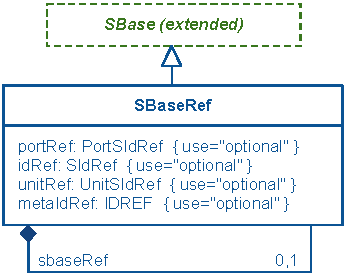
\includegraphics{figs/sbaseref-uml}
  \caption{The extensions of the \SBaseRef class.  The four attributes
    \token{portRef}, \token{idRef}, \token{unitRef} and \token{metaIdRef}
    are mutually exclusive; only one can have a value in a given object
    instance.  The recursive structure also allows referencing entities
    in submodels of submodels, to arbitrary depths, as described in the
    text.}
  \label{sbaseref-uml}
\end{figure}


\subsubsection{The attributes of \class{SBaseRef}}

The four different attributes on \SBaseRef are mutually exclusive: only
one of the attributes can have a value at any given time, and exactly
one must have a value in a given \SBaseRef object instance.  (Note that
this is true of the basic \SBaseRef class; however, derived classes such
as \ReplacedElement may add additional attributes and extend or override
the basic attributes and mechanisms.)

All of the attributes face the following common namespace issue.  As
discussed in more detail in \sect{namespaces}, attributes of type
\primtype{SId}, \primtype{UnitSId}, and \primtype{PortSId} need only be
unique on a per-\Model basis.  This means that an interpreter of the
SBML document must be able to determine the model to which
\token{idRef}, \token{unitRef}, and \token{portRef} attributes refer.
In addition, even though \primtype{ID} values are unique on per-document
level, the same SBML element may be instantiated in multiple submodels,
in any number of \Model objects, and therefore the \token{metaIdRef}
attribute must also know to which \Model instantiation it is referring.
Just exactly how this is done is something that is left up to the
classes that subclass \SBaseRef.  The sections that describe \Port,
\Deletion, \ReplacedElement and \ReplacedBy describe the approach taken
in each case.

Separately, readers may wonder why so many different alternatives are
necessary.  The reason is that in a given scenario, the referenced model
may be located in an external file beyond the direct control of the
modeler, and so the preferred methods of referencing the subobjects may
not be available.  \SBaseRef provides multiple alternatives so that a
variety of modeling scenarios can be supported.

It is also worth noting that SBaseRef classes may point to elements
from other SBML Level 3 packages.  One possibility is that the package
will define a new \SBase-derived class, which will inherit the \token{metaId}
attribute.  These metaIDs may be referenced by the \SBaseRef \token{metaIdRef}
attribute.  Another possibility is that the package will define a class,
and define an attribute for that class of the type SId or UnitSId.  Should
it do so, those elements may be referenced with the \token{idRef} or \token{unitRef}
attributes, respectively.  A final possibility is that the package will 
define a class with a child element from the core specification (as this 
package does with core '\Model' objects being children of the 
'\ListOfModelDefinitions' class).  In that case, that child element may be 
referenced by any of its IDs as if it was in its normal location in core.

Because referencing elements in other namespaces is allowed, all classes that
inherit from SBaseRef must declare what to do when the referenced element
is part of a namespace that the current interpreter does not understand, and
if there are any additional restrictions on referencing other namespaces.  Any
\SBaseRef objects which are not derived classes defer to their \SBaseRef-derived
parent for any such restrictions and rules.

\paragraph{The \fixttspace\token{portRef} attribute}
\label{sbaseref-portref}

The optional attribute \token{portRef} takes a value of type
\primtype{PortSIdRef}.  As its name implies, this attribute is used to
refer to a port identifier, in the case when the reference being
constructed with the \SBaseRef is intended to refer to a port on a
submodel.  The namespace of the \primtype{PortSIdRef} value is the set
of identifiers of type \primtype{PortSId} defined in the submodel, not
the parent model.


\paragraph{The \fixttspace\token{idRef} attribute}
\label{sbaseref-idref}

The optional attribute \token{idRef} takes a value of type
\primtype{SIdRef}.  As its name implies, this attribute is used to
refer to a regular identifier (i.e., the value of an \token{id}
attribute on some other object), in the case when the reference being
constructed with the \SBaseRef is intended to refer to an object that
does not have a port identifier.  The namespace of the \primtype{SIdRef}
value is the set of identifiers of type \primtype{SId} defined in the
submodel, not the parent model.


\paragraph{The \fixttspace\token{unitRef} attribute}
\label{sbaseref-unitref}

The optional attribute \token{unitRef} takes a value of type
\primtype{UnitSIdRef}.  This attribute is used to refer to the identifier
of a \UnitDefinition object.  The namespace of the \primtype{UnitSIdRef}
value is the set of unit identifiers defined in the submodel, not the
parent model.

Note that even though this attribute is of type \primtype{UnitSIdRef},
the reserved unit identifiers that are defined by SBML Level~3 (see
Section~3.1.10 of the SBML Level~3 Version~1 core specification) are
\emph{not} permitted as values of \token{unitRef}.  Reserved unit
identifiers may not be replaced or deleted.


\paragraph{The \fixttspace\token{metaIdRef} attribute}
\label{sbaseref-metaidref}

The optional attribute \token{metaIdRef} takes a value of type 
\primtype{IDREF}.  This attribute is used to refer to a \token{metaid}
attribute value on some other object, in the case when the reference
being constructed with the \SBaseRef is intended to refer to an object
that does not have a port identifier.  Since meta identifiers are
optional attributes of \SBase, all SBML objects have the potential to
have a meta identifier value.


\subsubsection{Recursive \class{SBaseRef} structures}
\label{sbaseref-recursive-sbaseref}

An \SBaseRef object may have up to one subcomponent named
\token{sBaseRef}, of type \SBaseRef (see \fig{sbaseref-uml}).  This
arrangement permits recursive structures to be constructed so that
objects inside submodels can be referenced.

The form of such recursive references must be as follows.  The
highest-level \SBaseRef object of such a chain (which will necessarily
be an object of class \Port, \Deletion, \ReplacedElement or \ReplacedBy,
because they are the only classes derived from the class \SBaseRef) must
refer to a \Submodel object in the containing model.  All child
\SBaseRef objects in the chain must refer to components inside the
\Model instance to which the \Submodel refers.

The following example may help clarify this.  Suppose that we want to
delete an object with the identifier \val{p1} inside the \Submodel
object identified as \val{sub\_m1}.  \fig{submodel-uml} shows that \Deletion
objects are placed inside a \ListOfDeletions within a \Submodel.  The 
following XML fragment illustrates how the constructs will look:

\begin{example}
<submodel id="sub_m1" modelRef="m1">
  <listOfDeletions>
    <deletion idRef="p1" />
  </listOfDeletions>
</submodel>
\end{example}

Suppose instead that the submodel \val{m1} from the previous example is
actually nested inside another submodel \val{m2}.  Then, we would have
the following:

\begin{example}
<listOfModelDefinitions>
  <modelDefinition id="m1">
    <listOfParameters>
      <parameter id="p1" value="3"/>
    </listOfParameters>
  </modelDefinition>
  <modelDefinition id="m2">
    <listOfSubmodels>
      <submodel id="sub_m1" modelRef="m1"/>
    </listOfSubmodels>    
  </modelDefinition>
  <modelDefinition id="m3">
    <listOfSubmodels>
      <submodel id="sub_m2" modelRef="m2">
        <listOfDeletions>
          <deletion idRef="sub_m1">
            <sBaseRef idRef="p1" />
          </deletion>
        </listOfDeletions>
      </submodel>
    </listOfSubmodels>    
</listOfModelDefinitions>
\end{example}

Finally, what if we needed to go further down into nested submodels?
The following example illustrates this:

\begin{example}
<listOfModelDefinitions> 
  <modelDefinition id="m1"> 
    <listOfParameters> 
      <parameter id="p1" value="3"/> 
    </listOfParameters> 
  </modelDefinition> 
  <modelDefinition id="m2"> 
    <listOfSubmodels> 
      <submodel id="sub_m1" modelRef="m1"/> 
    </listOfSubmodels>     
  </modelDefinition> 
  <modelDefinition id="m3"> 
    <listOfSubmodels> 
      <submodel id="sub_m2" modelRef="m2"/> 
    </listOfSubmodels>     
  </modelDefinition> 
  <modelDefinition id="m3"> 
    <listOfSubmodels> 
      <submodel id="sub_m3" modelRef="m3"> 
        <listOfDeletions> 
          <deletion idRef="sub_m2"> 
            <sBaseRef idRef="sub_m1"> 
              <sBaseRef idRef="p1" />
            </sBaseRef> 
          </deletion> 
        </listOfDeletions> 
      </submodel> 
    </listOfSubmodels>     
</listOfModelDefinitions> 
\end{example}


Although this use of nested \SBaseRef objects allows a model to refer to
components buried inside submodels, it is considered inelegant model
design.  It is better to promote any element in a submodel to a local
element if it can be predicted that containing models may need to
reference it.  However, if the submodel is fixed (e.g., if is in an
external file), then no other option may be available except to use
nested references.



% -----------------------------------------------------------------------------
\subsection{Conversion factors}
\label{conversion-factors}

%\draftnote{[MH] I have not looked at this section.}
In SBML Level~3 Version~1 Core, units of measurement are optional
information.  Modelers are required to write their models in such a way
that all conversions between units are explicitly incorporated into the
quantities, so that nowhere do units need to be understood and values
implicitly converted before use.  Given the Hierarchical Model
Composition package's design goal of compatibility with existing models
and files that may not be changeable, it is not an option to require
that all included models must be written in such a way that they are
numerically compatible with each other.  For example, if one submodel
defines how a species amount changes in time, and a second submodel
defines an initial assignment for that same species in terms of
concentration, something must be done to make the model as a whole
coherent without editing the submodels directly.  That is the purpose of
the conversion factor attributes on the \ReplacedElement and \Submodel
classes.


\subsubsection{Conversion factors involving \class{ReplacedElement}}

When an element in a submodel has been replaced by an element in a
containing model, old references to the replaced element are replaced by
references to the replacement element.  However, the mathematical
formulas associated with that replaced element may be in a different
scale than the ones used for the replacement element.  Correcting this is the purpose
of the \token{conversionFactor} attribute on \ReplacedElement objects.

There are two types of mathematical references possible in SBML:  assignments
to a variable, and the use of a variable in calculations.  In the former
case, when an assignment (an \InitialAssignment, \EventAssignment, \AssignmentRule,
or \RateRule) targets a replaced element, that formula should be 
multiplied by the conversion factor before being used.  In the latter
case, when a MathML <cn> element references the replaced element's ID, that
reference should be considered to be divided by the conversion factor.

For example, if a species has an initial assignment of $4x + 3$, and has
a conversion factor of $c$, the initial assignment formula becomes
$c (4x+3)$.  Conversely, if the $x$ has
been replaced and given a conversion factor of $c_x$, that initial
assignment formula would become $4((x/c_x)+3)$.  This holds true for any
mathematical equation in the model, including algebraic rules.  This
also means that if a value appears on the right and left-hand sides of
an equation, you must apply the conversion factor twice: if the rate
rule of $x$ is $4x+3$, it becomes $c_x(4(x/c_x) + 3)$.  (This
simplifies to $4x + 3c_x$, as you would expect---the $x$ is already in
the correct scale; it is only the $3$ that must be converted.)



\subsubsection{Conversion factors involving \class{Submodel}}

Most of the math in an SBML model may have arbitrary units, but there are
two exceptions to this rule:  time, and reaction extent.  While both of
these mathematical concepts may be scaled to arbitrary units, multiple
such scales in a single document are not allowed:  all references to
time assume a single scale, and all reactions are assumed to process
their reactants and products in the same way.

The \token{timeConversionFactor} and \token{extentConversionFactor} attributes 
on \Submodel dictate how time and reaction extent are to be converted to 
match the scale of the containing model.  As described in 
\sect{submodel-timeconversionfactor},
this includes the MathML csymbols
\token{time} and \token{delay}, as well as any \Delay, \KineticLaw, or
\RateRule objects which are \emph{not} replaced in the \Submodel.

The \token{conversionFactor} attributes on \Species and \Model objects defined
in SBML Level~3 Version~1 core are unrelated to the above conversion factors.  They
allow multiple substance scales to be converted to the single extent scale, so that
\Species may have different units from each other, even though the units of all
\KineticLaw elements are the same.  Because \Species are allowed to have different
units of substance, there is no need for a \token{substanceConversionFactor}
attribute on \Submodel.

To understand the rules, the entire list of classes and MathML elements
which are converted by these three factors (time, extent, and
replaced) in the SBML Level~3 Version~1 Core specification are provided
in \tab{sbml-conversions}.  Similar rules may be derived from other
packages that require any particular mathematics to be universal over 
a given \Model.

\newcommand{\sprd}[2]{\raisebox{-#1pt}[0pt][(#1pt * 2) + 4pt]{#2}}
\newcommand{\persymb}{\emph{Conversion factor for referenced object}}
\newcommand{\allat}{\emph{(All)}}

\begin{table}[bht]
  \rowcolors{2}{sbmlrowgray}{}
  \renewcommand{\arraystretch}{1.175}
  \begin{edtable}{tabular}{p{1.6in}p{2.3in}l}
    \toprule
    \textbf{Component}			& \textbf{Automatic conversion factor}\\
    \midrule
    \AlgebraicRule			& 1\\
    \AssignmentRule			& \persymb\\
    \Compartment			& 1\\
    \Constraint				& \emph{(Boolean:  none needed)}\\
    \Delay				& \token{timeConversionFactor}\\
    \EventAssignment			& \persymb\\
    \FunctionDefinition			& 1\\
    \InitialAssignment			& \persymb\\
    \sprd{4}{\KineticLaw} 		& \sprd{4}{$\frac{\token{extentConversionFactor}}{\token{timeConversionFactor}}$}\\
    \sprd{4}{MathML <cn> element}	& \sprd{4}{$\frac{1}{\textsf{\persymb}}$}\\
    \sprd{4}{MathML csymbol \token{time}} & \sprd{4}{$\frac{1}{\token{timeConversionFactor}}$}\\
    The \token{time} argument of a MathML csymbol \token{delay} function & \sprd{4}{\token{timeConversionFactor}}\\
    \Parameter				& 1\\
    \Priority				& 1\\
    \sprd{4}{\RateRule} 		& \sprd{4}{$\frac{\textsf{\persymb}}{\token{timeConversionFactor}}$}\\
    \Species 				& 1\\
    \SpeciesReference			& 1\\
    \Trigger				& \emph{(Boolean:  none needed)}\\
    \bottomrule
  \end{edtable}
  \caption{Conversion factors used for the different components defined
    by SBML Level~3 Core.}
  \label{sbml-conversions}
\end{table}

Any listed automatic conversion factor of '1' simply means that the given 
math is not converted.  Similarly, if a conversion factor is not defined,
it too defaults to '1', so that if (for example)
\token{extentConversionFactor} is defined but \token{timeConversionFactor} is
not, kinetic laws are converted according to the 
\token{extentConversionFactor}, 'divided by~1'.

Note that for the MathML <cn> element conversion,
the \token{SId} of a \Reaction references its \KineticLaw, meaning that if
the \KineticLaw was converted as in \tab{sbml-conversions}, its appearance
in MathML will also need to be converted by its inverse.  \AssignmentRule and \RateRule
\token{SId}s cannot appear in any MathML, and thus do not need to be checked
the same way.

Converting the formula of a \RateRule may involve a combination of conversion factors.
If the target of the \RateRule has been replaced
and given a \token{conversionFactor}, and its \Submodel has a defined 
\token{timeConversionFactor}, the formula must be multiplied by the \token{conversionFactor}
and divided by the \token{timeConversionFactor} before being used.

There is only one example of math that is assumed to be in the same scale
across a single SBML model but that cannot be converted according to
these conversion factors:  the math associated with the \Priority
subcomponent of \Event objects.  When comparing priority expressions 
across submodels,
they are all assumed to be on the same scale relative to each other.
Thus, if one submodel had priorities set on a scale of 0 to 10 and another had
priorities set on a scale of -100 to 100, the only way to reconcile the 
two would be to replace all events which had priorities on one scale with
events with priorities on the new scale.
The same would be true of math defined in any other Level~3 package
without the unit type of extent or time, but which was assumed to
be universally consistent across multiple objects in the SBML model.
To correctly compose models with different scales of such objects using
this package, every nonconformant object would need to be replaced and
given an explicit conversion factor, or that package would have to
extend this Hierarchical Model Composition package to define a new
attribute on Submodel that could be used to automatically convert all
such elements in the submodel with that unit type.


\clearpage

% -----------------------------------------------------------------------------
\subsection{Namespace scoping rules for identifiers}
\label{namespaces}

In the Hierarchical Model Composition package, as in SBML Level~3
Version~1 Core, the \Model object contains the main components of an
SBML model, such as the species, compartments and reactions.  The
package adds the ability to put \emph{multiple} models inside an SBML
document, and therefore must define the scope of identifiers in such a
way that identifier collisions are prevented.  In this section, we
describe the scoping rules for all of the types and classes defined in
Sections~\ref{new-primitive-types}--\ref{sbaseref-class}.

\begin{enumerate}

\item A shared namespace exists for \primtype{SId} values defined at the
  level of the SBML document.  This namespace applies to the identifiers
  (i.e., values of \token{id} attributes) of all \Model and
  \ExternalModelDefinition objects within the SBML document.  (An
  \ExternalModelDefinition object references a model elsewhere, so in
  this sense, both \Model and \ExternalModelDefinition are types of
  models.)  The identifier of every \Model and \ExternalModelDefinition
  object must be unique across the set of all such identifiers in the
  document.  The namespace is limited to that SBML document, and is not
  shared with any other SBML document, even if that document is
  referenced via an \ExternalModelDefinition.  This namespace is known
  as \emph{the model namespace of the document}.

\item The namespace for \primtype{SId} identifiers defined \emph{within}
  a \Model object used in Hierarchical Model Composition follows the
  same rules as those defined in SBML Level~3 Core for plain \Model
  objects.  That is, the scope of the identifiers is limited to the
  enclosing \Model object.  This means that two or more \Model objects
  in the same document may reuse the same object identifiers inside of
  them; the identifiers do not need to be unique at the level of the
  SBML document.  (For example, two model definitions could use the same
  \primtype{SId} value for \Parameter objects within their respective
  contents.  Note, however, that this does \emph{not} imply that the two
  objects are equated with each other!)  An implication of this rule is
  that to fully locate an object, one must know not only the object's
  identifier, but also the identifier of the model in which it is
  located.  This is known as the \emph{object namespace of the model}.  

\item The identifier of every \UnitDefinition object must be unique
  across the set of all such identifiers in the \Model to which they
  belong.  (This is the same as in SBML Level~3 Version~1 Core.)
  Similar to the case above, an implication of this rule is that to
  fully locate a user-defined unit definition when there are multiple
  models in an SBML document, one must know not only the unit
  definition's identifier, but also the identifier of the model in which
  it is located.  This namespace is referred to as the 
  \emph{unit namespace of the model}.

\item The Hierarchical Model Composition package defines a new kind of
  component: the \emph{port}, represented by \Port objects.  The
  identifier of every \Port object must be unique across the set of all
  such identifiers in the \Model object to which they belong.  Again, an
  implication of this rule is that to fully locate a port when there are
  multiple models in an SBML document, one must know not only the port's
  identifier, but also the identifier of the model in which it is
  located.  This namespace is referred to as the 
  \emph{port namespace of the model}.

\item \Reaction objects introduce a local namespace for \LocalParameter
  objects.  These objects cannot be referenced from outside a given
  reaction definition.  For the Hierarchical Model Composition package,
  the implication is that the the \SBaseRef class
  (\sect{sbaseref-class}) cannot reference reaction local parameters
  simply by their identifiers (i.e., the value of their \token{id}
  attribute).  However, the \LocalParameter objects \emph{can} be given
  meta identifiers (a value for their \SBase-derived \token{metaid}
  attribute), and be referenced using those.  This namespace is
  referred to as the \emph{local namespace of the reaction}.

% FIXME need move this somewhere else:
% 
%   If replaced, it must be by an element in the normal element namespace of
%   a model (such as a global Parameter).  Old references to that replaced
%   LocalParameter will then point to the new replacement element.  If a
%   LocalParameter is deleted from a Reaction whose KineticLaw used it in
%   its math, that KineticLaw may still be valid if there was an element
%   in the element namespace of the model with that same id to which it
%   can now refer (in other words, if the LocalParameter shadowed a global
%   parameter).


\end{enumerate}

The following example may clarify some of these rules.  Suppose a given
SBML document contains a \Model object having the identifier \val{mod1}.
This \Model cannot contain another object with the same identifier
(e.g., it could not have a \Parameter object with the identifier
\val{mod1}), nor can there be any other \Model or
\ExternalModelDefinition object identified as \val{mod1} within the
same SBML document.  The first restriction is simply the regular SBML
rule about uniqueness of identifiers throughout a \Model object; the
second restriction is due to point (1) above.  On the other hand, there
could be a second \Model object in the same document containing a
component (e.g., a \Parameter) with the identifier \val{mod1}.  This
would not conflict with the first \Model identifier (because the
\Parameter would be effectively hidden at a lower level within the
second \Model).

